\section{Methodology Descripttion}
\subsection{ETL Data for Dataset 1}
\subsubsection{Data Sources}
For the data extraction process, we utilized product reviews and specifications from the \href{https://pricebaba.com/}{pricebaba} website. This site offers a comprehensive range of products, including mobile phones, laptops, televisions, and other electronic devices. For this research, we initially focused exclusively on mobile phone data. The site provides detailed product information and expert reviews, making it a valuable data source for training and evaluating review generation models.
\\\\
The reviews are structured as shown in Figure \ref{fig:pricebaba-review-structure}, Each review includes a detailed description of the product, pros and cons, and descriptions focused on various features such as the camera, battery, screen, etc. Additionally, Figure \ref{fig:pricebaba-spec-structure} shows that the product specifications are structured in tables and sub-tables, facilitating data extraction.
\begin{figure}[H]
    \centering
    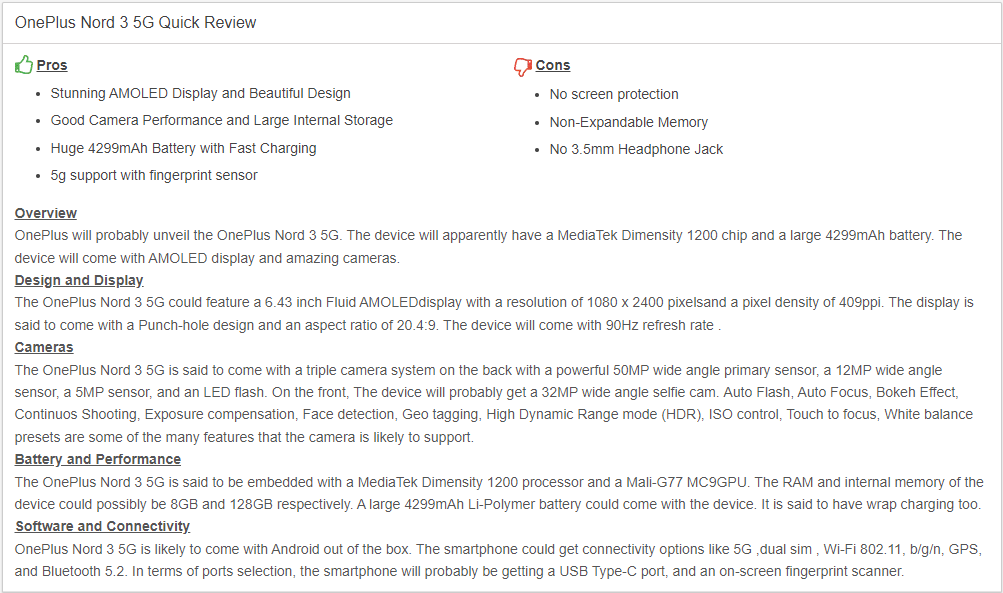
\includegraphics[width=12cm]{images/pricebaba_review_structure.png}
    \caption{pricebaba reviews structure \cite{OnePlusNord35G2023}}
    \label{fig:pricebaba-review-structure}
\end{figure}
\begin{figure}[H]
    \centering
    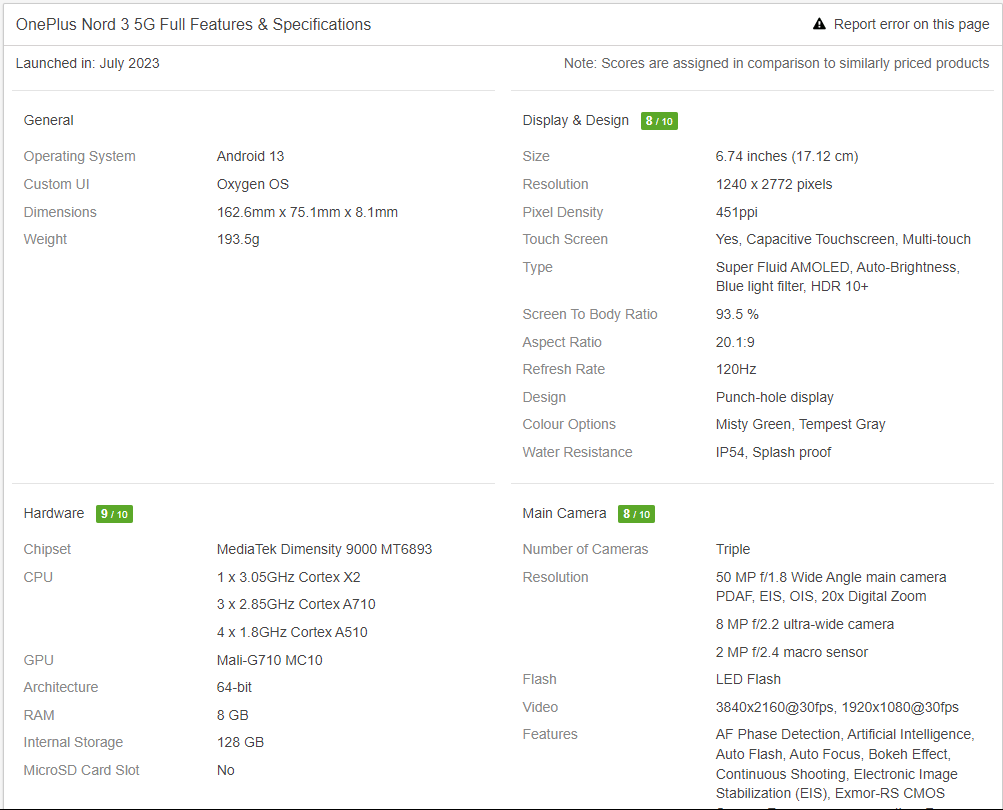
\includegraphics[width=12cm]{images/pricebaba_spec_structure.png}
    \caption{pricebaba specifications structure \cite{OnePlusNord35G2023}}
    \label{fig:pricebaba-spec-structure}
\end{figure}
To achieve data extraction, we will use the technique of web scraping, which involves extracting information from web pages to formatting to store it on a database. In this case, we will extract reviews and specifications of mobile phones from the pricebaba website and store them in JSON format for subsequent processing. This process yielded a dataset of reviews and specifications for 7400 mobile phones, serving as the initial database for cleaning and formatting.

\subsubsection{Data Format}
The chosen format for data representation is JSON, as this format allows for structured and easy-to-process data representation. Two JSON files will be used to represent the data: one for the reviews and another for the product specifications. This last one will contains two parts per product: the key values, which means the most important data of the product, and the full specifications. Each JSON file will contain an array of objects, where each object will represent a product along with its respective reviews or specifications. The structure of the JSON files is outlined below:
\newpage
\begin{lstlisting}[style=jsonstyle, frame = single, caption=JSON Data Format Product specification, label=code:json-data-format]
{
    "url": {
        "keys_specifications": [],
        "full_specifications": [
            "Launch Date": "Launch Date",
            "General": {
                "subcategories1": [
                    "value1"
                    ],
                "subcategories2": [
                    "value1",
                    "value2"
                    ],
                ...
            },
            "Characteristic1": {
                "subcategories1": [
                    "value1"
                    ],
                "subcategories2": [
                    "value1",
                    "value2"
                    ],
                ...
            },
            "Characteristic2": {
                "subcategories1": [
                    "value1"
                    ],
                "subcategories2": [
                    "value1",
                    "value2"
                    ],
                ...
            },
            ...
        ]
    },
}
\end{lstlisting}
\newpage
\begin{lstlisting}[style=jsonstyle, frame = single, caption=JSON Data Format reviews, label=code:json-data-format]
{
    "url": {
        "text": {
            "Characteristic1": ["Description1"],
            "Characteristic2": ["Description2"],
            ...
        },
        "Pros": [
            "Pro 1",
            "Pro 2",
            "Pro 3"
        ],
        "Cons": [
            "Con 1",
            "Con 2",
            "Con 3"
        ]
    },
}
\end{lstlisting}

\subsubsection{Data Normalization}
After structuring the data into the two JSONs format, normalization is carried out. This involves evaluating the keys of the objects, cleaning keys that contain spaces, transforming keys, subkeys, and values to lowercase, replacing `\&` with `and`, and reordering keys that include `and` to maintain a logical order. For instance, the key `Display \& Design` was changed to `Design and Display`. This process will be applied to both the reviews and specifications JSONs. 

\subsubsection{Merging Data}
The next step is to merge the reviews and specifications JSONs into a single JSON file. This will involve matching the reviews and specifications of each product based on the product's URL. This process will result in a single JSON file that contains all the information for each product, including the reviews and specifications. This merged JSON file will be used for further processing.

\subsubsection{Data Removal}
Once all data is normalized and merged, the process of removing duplicates and unnecessary data begins. This will include deleting reviews that contain no value in the `text` key, specifications that only have the value `General', or reviews that only contain the value `Overview'. This is because our goal is to conduct detailed product reviews based on their distinct characteristics, rather than in a generalized manner.

\subsubsection{Split data}
Once the data has been cleaned and structured, the dataset is divided into three sets: training, and testing. For this, an 80\% portion will be allocated for training and 20\% for testing. This ensures that the models are trained with a sufficient amount of data and evaluated appropriately.

\subsection{ETL Data for Dataset 2}
\subsubsection{Data Sources}
This dataset will be use to applied a cross-validation technique to evaluate the models. The data will be obtained for an existing dataset that is not product-based, but it is focused on structured data in JSON format. The dataset is QTSUMM \cite{zhao2023qtsummqueryfocusedsummarizationtabular}, which contains the columns: table, which contains JSON format data; query, which is the `keys' the model will use to generate the output; and summary, the expected output. The dataset is structured as shown in Figure \ref{fig:qsumm-structure}, where each object contains the columns especified before. This dataset will be used to generate prompts for the models to evaluate their performance.

\begin{figure}[H]
    \centering
    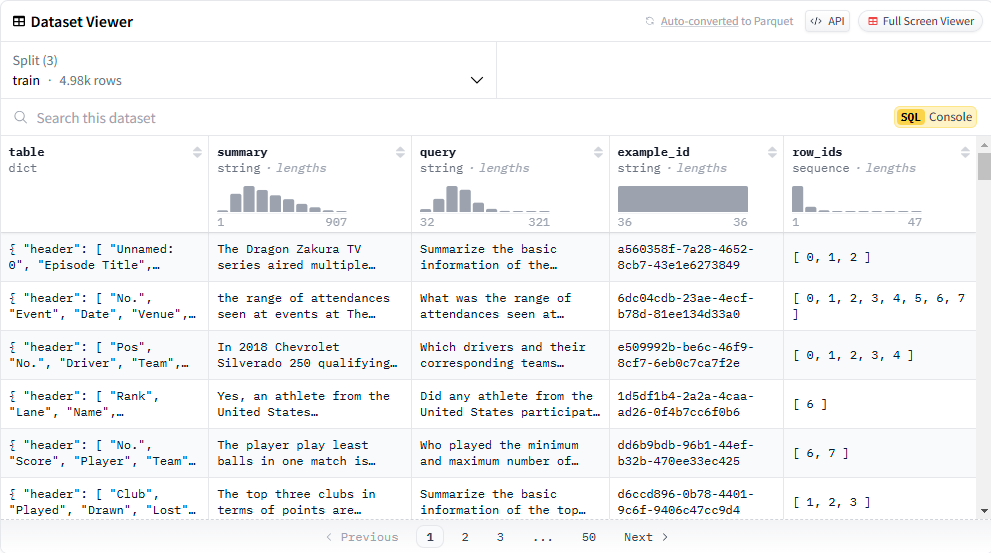
\includegraphics[width=12cm]{images/qsumm_structure.png} 
    \caption{QTSUMM dataset structure \cite{zhao2023qtsummqueryfocusedsummarizationtabular}}
    \label{fig:qsumm-structure}
\end{figure}

\subsection{Data formatting}
For the QTSUMM dataset, it will be necessary add a column to stores the `prompts' that will be used to evaluate the models. This column will be generated based on the `table', `query' and `summary' columns of the dataset. In the section \ref{subsubsec:prompt-structuration} the process of structuring the prompts will be explained in detail. The final dataset will be used to evaluate the models. 

\subsection{Prompt structuration}\label{subsubsec:prompt-structuration}
The prompt structure will be adapted for both datasets to ensure the models are capable of generating expected outputs based on the input data. Eventhoug the explanations of the prompts will be separated in the followings sections.

\subsubsection{Prompt structuration for Dataset 1}
Once the JSONs for reviews and specifications have been cleaned, the next step is to structure the instructions that will be used to train the models. These instructions will form the final dataset. For this purpose, instructions with the following structure will be created:
\begin{lstlisting}[style=textstyle, frame = single, caption=Prompt structuration, label=code:prompt-structuration]
"Given following json that contains specifications of a product, generate a review of the key characteristics with json format. Follow the structure on Keys to write the Output: 
### Product: Product for JSON specifications
### Keys: Combination of the keys of the JSON reviews
### Output: reviews for JSON reviews accordingly to the keys"
\end{lstlisting}
it means that instructions will be generated for each permutation of the review keys. For example, if there is a review with the keys Design and Display', Camera', Battery', Performance', Software', i' instructions are chosen from the possible combinations of these keys, where i' is the number of instructions desired to be generated. This approach ensures that the model generates reviews according to the different characteristics of the products. An example of key selection could be that if a product has the keys Design and Display', Camera', Battery', Performance', Software', then the keys Design and Display', Camera' might be selected to generate one instruction, and for another instruction for the same product, the keys Design and Display', Battery' might be selected, and so on.
\\\\
With these combinations of keys for generating instructions, from the original 7,400 data points, 60,700 instructions are obtained that will be used to train the models. These instructions are the final dataset, which is available on \href{https://huggingface.co/datasets/kokujin/json_data_luis}{Hugginface}.

\subsubsection{Prompt structuration for Dataset 2}
For the QTSUMM dataset, the `prompts' column will be filled with data as follows:
\newpage
\begin{lstlisting}[style=textstyle, frame = single, caption=Prompt structuration, label=code:prompt-structuration]
"Given following json that contains specifications of a product, generate a review of the key characteristics with json format. Follow the structure on Keys to write the Output: 
### Product: Column table of JSON specifications
### Keys: Column query of the dataset
### Output: Column summary of the dataset"
\end{lstlisting}
The `prompt' as shown have the same format for both dataset, but the data used to fill them are different. This will allows the models understands the instructions no matter the dataset used to train or evaluate them.


\subsection{Model Fine-Tuning}
\subsubsection{Hyperparameter Selection}
Due to the fact that the Large Language Models (LLMs) to be used are already pretrained, the hyperparameters selected will be those used for the fine-tuning process of the models. Additionally, due to computational limitations, hyperparameters that fit the capabilities of the machine on which the fine-tuning process will be conducted will be selected. For this purpose, the hyperparameters from Table \ref{table:hyperparameters} will be chosen.
\begin{table}[H]
    \centering
    \begin{tabular}{|c|c|}
        \hline
        \textbf{Hyperparameter} & \textbf{Value} \\
        \hline
        Learning Rate & 2e-4 \\
        Batch Size & 2 \\
        Epochs & 2 \\
        max\_grad\_norm & 0.3 \\
        lr\_scheduler\_type & cosine\\
        gradient\_accumulation\_steps & 3 \\
        weight\_decay & 0.001 \\
        warmup\_ratio & 0.03 \\
        lr\_scheduler\_type & cosine \\
        optim & paged\_adamw\_32bit \\
        max\_seq\_length & 1000 \\
        lora\_r & 64 \\
        lora\_alpha & 16 \\
        lora\_dropout & 0.1\\
        \hline
    \end{tabular}
    \caption{Hyperparameters Selection}
    \label{table:hyperparameters}
\end{table}
The choice of `max\_seq\_length` is based on prior estimation of the average token length of the reviews, which was found to be 900 tokens. To achieve this, it was necessary to iterate through each prompt and use a tokenizer. Furthermore, the `BitsAndBytesConfig` library from Hugging Face's `transformers` has been utilized for model optimization. These additional hyperparameters are shown in Table \ref{table:hyperparameters-bitsandbytes}.
\begin{table}[H]
    \centering
    \begin{tabular}{|c|c|}
        \hline
        \textbf{Hyperparameter} & \textbf{Value} \\
        \hline
        bnb\_4bit\_compute\_dtype & float16 \\
        bnb\_4bit\_quant\_type & nf4 \\
        use\_nested\_quant & False \\
        \hline
    \end{tabular}
    \caption{Hyperparameters Selection BitsAndBytes}
    \label{table:hyperparameters-bitsandbytes}
\end{table}

\subsection{Fine-Tuning Process}
For the fine-tuning process, three different models will be used to generate reviews: \texttt{StructLM-7B}, \texttt{Mistral\_Instruct-7B}, and \texttt{Llama2-7B}. This process will be divided into two parallel steps. In the first step, the three models will be trained with a dataset of product information obtained from Alibaba. In the second step, three models with the same architectures will be trained using the QTSUMM dataset. The training will utilize the hyperparameters specified in the previous section.
\\\\
To ensure efficient fine-tuning, the models will be trained with Hugging Face's \texttt{transformers} library, a powerful and accessible tool for model training. The process will be run on a machine equipped with a 4070 Ti Super GPU for optimal performance. By the end, there will be six fine-tuned models: two \texttt{Llama2-7B} models (one trained on Alibaba data and one on QTSUMM), two \texttt{Mistral\_Instruct-7B} models (one trained on each dataset), and two \texttt{StructLM-7B} models (also one per dataset).

\subsection{Model Evaluation}\label{subsec:model-evaluation}
Once the models have been fine-tuned, they are evaluated using the test data. For this purpose, metrics such as BLEU, METEOR, and ROUGE were used. These metrics compare the reviews generated by the models with the actual product reviews, thereby assessing the quality of the reviews produced by the models and determining which model best fits the test data.
\\\\
Additionally, the model's propensity to hallucinate or inaccurately include critical information in reviews will be assessed. This evaluation will leverage a model-based scoring mechanism, specifically the \href{https://huggingface.co/prometheus-eval/prometheus-7b-v2.0}{Prometheus} model \cite{kim2024prometheus2opensource}, an open-source large language model (LLM) designed to evaluate various capabilities of other models. For the trained models, the key metrics under consideration will be faithfulness and correctness. To conduct this evaluation, a prompt must be constructed following the structured guidelines outlined in the paper \cite{kim2024prometheus2opensource}, with a focus on assessing both faithfulness\ref{code:estructured-faithfullness} and correctness\ref{code:estructured-correctness}.

\begin{lstlisting}[style=python, frame = single, caption=Prompt estructured correctness, label=code:estructured-correctness]
    instruction = f"""Your task is to evaluate the generated answer and reference answer for the query: {Prompt}"""
    response = f"""{Predicted}""" 
    reference_answer = f"""{Original}"""
    rubric = {
        "criteria": "Is the model proficient in generate a coherence response",
        "score1_description": "If the generated answer is not relevant to the user query and reference answer.",
        "score2_description": "If the generated answer is according to reference answer but not relevant to user query.",
        "score3_description": "If the generated answer is relevant to the user query and reference answer but contains mistakes.",
        "score4_description": "If the generated answer is relevant to the user query and has the exact same metrics as the reference answer, but it is not as concise.",
        "score5_description": "If the generated answer is relevant to the user query and fully correct according to the reference answer."}

    ABS_SYSTEM_PROMPT = "You are a fair judge assistant tasked with providing clear, objective feedback based on specific criteria, ensuring each assessment reflects the absolute standards set for performance."

    ABSOLUTE_PROMPT = f"""###Task Description:
    An instruction (might include an Input inside it), a response to evaluate, a reference answer that gets a score of 5, and a score rubric representing a evaluation criteria are given.
    1. Write a detailed feedback that assess the quality of the response strictly based on the given score rubric, not evaluating in general.
    2. After writing a feedback, write a score that is an integer between 1 and 5. You should refer to the score rubric.
    3. The output format should look as follows: "Feedback: (write a feedback for criteria) [RESULT] (an integer number between 1 and 5)"
    4. Please do not generate any other opening, closing, and explanations.

    ###The instruction to evaluate:
    {instruction}

    ###Response to evaluate:
    {response}

    ###Reference Answer (Score 5):
    {reference_answer}

    ###Score Rubrics:
    {rubric}

    ###Feedback: """

    user_content = ABS_SYSTEM_PROMPT + "\n\n" + ABSOLUTE_PROMPT # Fill the prompt with your data

    messages = [
        {"role": "user", "content": user_content},
    ]
\end{lstlisting}

\begin{lstlisting}[style=python, frame = single, caption=Prompt estructured faithfullness, label=code:estructured-faithfullness]
    instruction = f"""If the Generate answer has information from the context and also from the Existing answer."""
    response = f"""{Predicted}"""
    reference_answer = f"""{Original}"""
    rubric = {
        "score1_description": "If the generated answer is not having similarities from the context and also with existing answer.",
        "score2_description": "If the generated answer is having information from the context but not from existing answer.",
        "score3_description": "If the generated answer is having relevant information from the context and some information from existing answer but have additional information that do not exist in context and also do not in existing answer.",
        "score4_description": "If the generated answer is having relevant information from the context and some information from existing answer.",
        "score5_description": "If the generated answer is having relevant information from the context and all the information from existing answer."}

    ABS_SYSTEM_PROMPT = "You are a fair judge assistant tasked with providing clear, objective feedback based on specific criteria, ensuring each assessment reflects the absolute standards set for performance."

    ABSOLUTE_PROMPT = f"""###Task Description:
    An instruction (might include an Input inside it), a response to evaluate, a reference answer that gets a score of 5, and a score rubric representing a evaluation criteria are given.
    1. Write a detailed feedback that assess the quality of the response strictly based on the given score rubric, not evaluating in general.
    2. After writing a feedback, write a score that is an integer between 1 and 5. You should refer to the score rubric.
    3. The output format should look as follows: "Feedback: (write a feedback for criteria) [RESULT] (an integer number between 1 and 5)"
    4. Please do not generate any other opening, closing, and explanations.
    5. Only evaluate on common things between generated answer and reference answer. Don't evaluate on things which are present in reference answer but not in generated answer.

    ###The instruction to evaluate:
    {instruction}

    ###Context:
    {Prompt}

    ###Existing answer (Score 5):
    {reference_answer}

    ###Generate answer to evaluate:
    {response}

    ###Score Rubrics:
    {rubric}

    ###Feedback: """

    user_content = ABS_SYSTEM_PROMPT + "\n\n" + ABSOLUTE_PROMPT # Fill the prompt with your data

    messages = [
        {"role": "user", "content": user_content},
    ]
\end{lstlisting}

\subsection{Cross-Validation}
To finish the evaluation process, the models will be evaluated in a cross-validation manner, where the models trained on the Alibaba dataset will be evaluated using the QTSUMM dataset, and vice versa. This will allow for a comprehensive evaluation of the models' performance across different datasets. To evaluate the performance for the outputs generated by the models, it will be used the metrics explained in the previous section \ref{subsec:model-evaluation}.

\subsection{Resume}
This section provides a detailed overview of the methodology used for generating product reviews on e-commerce platforms using Large Language Models (LLMs). It describes the entire process from data collection and preparation, where data was generated from scratch, meticulously cleaned, and structured for further processing.
\\\\
The section continues by detailing the model tuning techniques, including the selection of hyperparameters and optimization methods, tailored to match the computational limits of the hardware. This phase was essential for adapting the models to produce relevant product reviews. The effectiveness of these fine-tuned models was then measured using evaluation metrics such as BLEU, METEOR, and ROUGE to assess the quality of generated reviews against actual product reviews.